\chapter{Implementation}
\begingroup
\justifying
\setlength{\parindent}{0pt}
\setstretch{1.5}
\setlength{\parskip}{0.5\baselineskip}
\titlespacing{\chapter}{0pt}{0pt}{0pt}
\titlespacing{\section}{0pt}{0pt}{0pt}

\section{Project Architecture}

The repository is organized into five major modules:
\begin{itemize}
    \item \texttt{contracts/}: Solidity contracts for election control, voter registry, and verifier adapters.
    \item \texttt{circuits/}: Circom circuits for vote and tally proofs.
    \item \texttt{frontend/}: voter and administrator web clients, including browser-side cryptographic helpers.
    \item \texttt{crypto/}: Python cryptographic implementation for BabyJubJub ElGamal and tally utilities.
    \item \texttt{test/} and \texttt{tests/}: JavaScript/Hardhat and Python/Pytest verification suites.
\end{itemize}

This modularity allows independent testing of smart-contract logic, cryptographic primitives, and user-facing flows.

Figure \ref{fig:system-architecture} illustrates the implementation layering and data movement between components.

\begin{figure}[htbp]
\centering
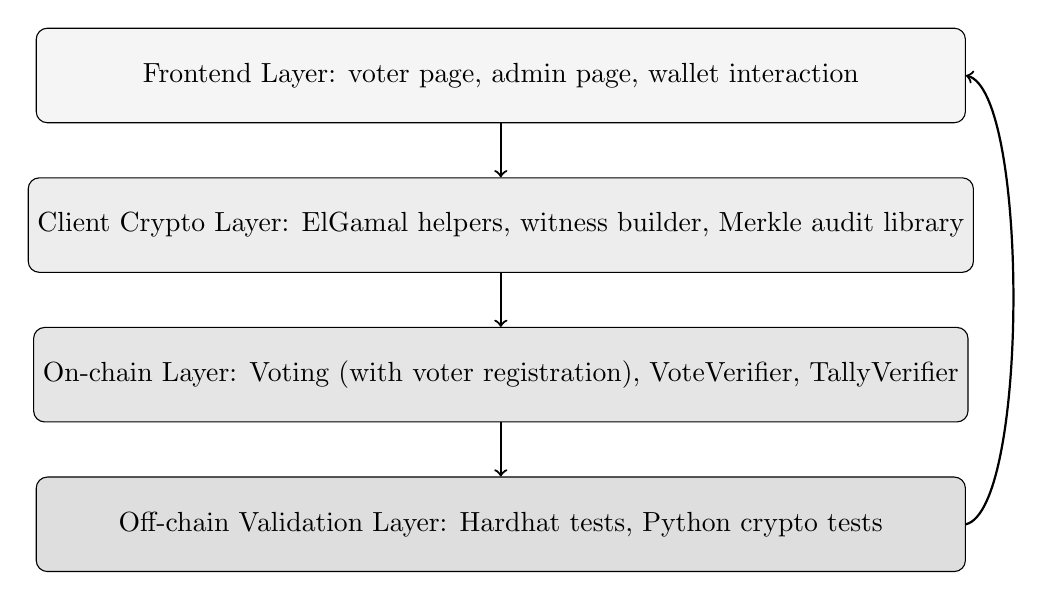
\begin{tikzpicture}[x=1cm,y=1cm]
    \node[draw, rounded corners, minimum width=11.8cm, minimum height=1.2cm, fill=gray!8] (ui) at (0,0) {Frontend Layer: voter page, admin page, wallet interaction};
    \node[draw, rounded corners, minimum width=11.8cm, minimum height=1.2cm, fill=gray!14] (crypto) at (0,-1.9) {Client Crypto Layer: ElGamal helpers, witness builder, Merkle audit library};
    \node[draw, rounded corners, minimum width=11.8cm, minimum height=1.2cm, fill=gray!20] (chain) at (0,-3.8) {On-chain Layer: Voting (with voter registration), VoteVerifier, TallyVerifier};
    \node[draw, rounded corners, minimum width=11.8cm, minimum height=1.2cm, fill=gray!26] (offchain) at (0,-5.7) {Off-chain Validation Layer: Hardhat tests, Python crypto tests};

    \draw[->, thick] (ui) -- (crypto);
    \draw[->, thick] (crypto) -- (chain);
    \draw[->, thick] (chain) -- (offchain);
    \draw[->, thick] (offchain.east) .. controls +(0.8,0.2) and +(0.8,-0.2) .. (ui.east);
\end{tikzpicture}
\caption{Implementation Architecture and Verification Loop}
\label{fig:system-architecture}
\end{figure}

\section{Smart Contract Design}

\subsection{Core Contract Responsibilities}

The voting contract is responsible for:
\begin{itemize}
    \item election initialization and candidate registration;
    \item lifecycle transition enforcement;
    \item vote acceptance conditioned on proof verification and voter eligibility;
    \item tally finalization conditioned on proof verification and consistency checks;
    \item Merkle-root publication for post-election audit.
\end{itemize}

Voter registration and one-vote enforcement are handled directly within the Voting contract, eliminating a separate registry dependency. Verifier contracts expose on-chain Groth16 verification interfaces.

\subsection{On-Chain Data Model}

Key on-chain structures include candidate records, per-voter vote metadata (commitment and ciphertext hash), and global commitment array. Ciphertext payload itself is emitted as event data to reduce storage cost while preserving off-chain reconstructability.

\subsection{Lifecycle Safeguards}

Contract modifiers enforce role and state restrictions. Invalid phase transitions, unauthorized calls, duplicate votes, and malformed proof submissions are rejected before state mutation.

Table \ref{tab:module-responsibility} summarizes how major modules split responsibilities.

\begin{table}[htbp]
\centering
\small
\caption{Module Responsibility Summary}
\label{tab:module-responsibility}
\begin{tabular}{L{3.0cm} L{4.0cm} L{5.8cm}}
\toprule
Module & Primary Input & Responsibility \\
\midrule
Voting contract & Proof calldata, commitments, tally outputs & Enforce lifecycle and accept/reject transitions by verification outcome. \\
Vote circuit & Candidate choice, salt, ciphertext components & Prove ballot legality and commitment/ciphertext consistency. \\
Tally circuit & Aggregated ciphertexts, secret key witness & Prove decryption correctness and total consistency. \\
Voter frontend & Candidate selection + wallet signature & Generate encrypted ballot and vote proof; store verification receipt. \\
Admin frontend & Encrypted vote events + admin key & Aggregate/decrypt tally, generate ZKP3, build/export audit bundle. \\
\bottomrule
\end{tabular}
\end{table}

\section{Circuit Implementation}

\subsection{Vote Circuit}

The vote circuit integrates Poseidon commitment checks, candidate range checks, one-hot encryption consistency checks, and ciphertext-hash binding. It is compiled with a fixed candidate cardinality parameter in current project configuration.

\subsection{Tally Circuit}

The tally circuit verifies key ownership relation, decryption correctness for aggregated ciphertexts, and sum consistency against total votes. Public signals are exported and consumed by the Solidity verifier.

\subsection{Artifact Pipeline}

Proof generation follows the standard Groth16 flow: circuit compilation, trusted setup artifacts, witness construction, proof generation, and verifier calldata export \cite{circomdocs,snarkjs}. Contract-side verification executes with precompiled pairing checks.

\section{Frontend Engineering Workflow}

\subsection{Voter Interface}

The voter page executes the following sequence:
\begin{enumerate}
    \item initialize cryptographic runtime and contract connections;
    \item fetch candidate list and election state;
    \item on candidate selection, generate ciphertexts and commitment;
    \item generate vote proof and prepare calldata;
    \item submit transaction through wallet;
    \item persist local receipt for later anonymous verification.
\end{enumerate}

\subsection{Administrator Interface}

The administrator page performs:
\begin{enumerate}
    \item encrypted vote event retrieval;
    \item ciphertext reconstruction and homomorphic aggregation;
    \item decryption and candidate result extraction;
    \item tally proof generation and contract submission;
    \item deterministic commitment Merkle-tree construction;
    \item audit-bundle export and local cache.
\end{enumerate}

\subsection{Audit Utility Module}

The audit utility in \texttt{frontend/lib/audit.js} centralizes:
\begin{itemize}
    \item bytes32 normalization;
    \item Merkle tree construction with duplicate-last odd handling;
    \item proof generation and verification;
    \item election-key namespace generation for local storage isolation.
\end{itemize}

This separation reduces logic duplication and improves testability.

\section{Testing and Validation Strategy}

\subsection{Contract-Level Tests}

Hardhat tests cover role control, lifecycle transitions, valid/invalid voting attempts, and tally submission behavior with Groth16 proofs. End-to-end scenarios include realistic proof generation and verifier invocation.

\subsection{Cryptographic Unit Tests}

Pytest cases validate curve arithmetic invariants, key generation, encryption/decryption correctness, homomorphic addition, one-hot vote encoding semantics, and bounded discrete-log solving.

\subsection{Engineering Observations}

The dual test stack provides coverage at both the contract protocol layer and the cryptographic primitive layer, giving high confidence in isolated module correctness. However, integration testing revealed several boundary conditions worth noting for future development.

First, the most brittle integration point is the mapping between circuit public signals and Solidity function parameters. Because snarkjs exports proof calldata in a specific encoding, any mismatch in signal ordering between the circuit definition and the contract's expected \texttt{pubSignals} array causes silent proof rejection rather than a descriptive error. This was addressed by careful alignment during circuit compilation, but requires maintenance discipline whenever circuits are recompiled.

Second, browser-side proof generation is resource-intensive. During development, memory pressure caused WASM crashes on devices with less than 4 GB available RAM. The voter interface should therefore include progress indicators and graceful error messages for proof generation failures.

Third, the ElGamal tally decryption relies on bounded discrete-log recovery (baby-step giant-step). If an election receives more votes than the precomputed table bound, decryption silently fails. This bound must be documented and enforced during deployment configuration.

\section{Deployment Notes}

Local deployment uses a Hardhat node and a Python-served static frontend. The deployment script (\texttt{scripts/deploy.js}) generates \texttt{frontend/config.js} automatically, which is required before the frontend pages can interact with the deployed contracts.

For testnet or mainnet deployment, the following additional steps apply:
\begin{itemize}
    \item Configure \texttt{.env} with the deployer private key and the target network RPC URL before running the deploy script.
    \item Ensure the \texttt{frontend/zk/} directory contains the compiled WASM witness generators and proving key files (\texttt{.zkey}) corresponding to the deployed verifier contracts.
    \item Configure MetaMask in the voter and administrator browsers to point to the correct network (chain ID must match the deployment target).
    \item The trusted setup artifacts (\texttt{build/pot16\_final.ptau} and circuit-specific \texttt{.zkey} files) must be kept consistent with the deployed verifier contracts. Recompiling circuits without redeploying verifiers will cause all proof submissions to fail.
\end{itemize}

The dependency on trusted setup artifacts and frontend configuration files is explicitly documented in repository instructions \cite{hardhat,solidity,openzeppelin}.

\section{Chapter Summary}

This chapter translated the protocol design into concrete software modules and execution paths. The key result is implementation traceability: every major protocol claim in Chapter 3 is mapped to explicit contract logic, circuit constraints, frontend operations, and automated tests. Chapter 5 evaluates whether this implementation meets the stated requirements, reports performance characteristics, and identifies residual security gaps.

\endgroup

